\documentclass{article}

\usepackage{fullpage,latexsym,picinpar,amsmath,amsfonts,graphicx}

           

%%%%%%%%%%%%%%%%%%%%%%%%%%%%%%%%%%%%%%%%%%%%%%%%%%%%%%%%%%%%%%%%%%%%%%%%%%%%%%%%%%%
%%%%%%%%%%%  LETTERS 
%%%%%%%%%%%%%%%%%%%%%%%%%%%%%%%%%%%%%%%%%%%%%%%%%%%%%%%%%%%%%%%%%%%%%%%%%%%%%%%%%%%

\newcommand{\barx}{{\bar x}}
\newcommand{\bary}{{\bar y}}
\newcommand{\barz}{{\bar z}}
\newcommand{\bart}{{\bar t}}

\newcommand{\bfP}{{\bf{P}}}

%%%%%%%%%%%%%%%%%%%%%%%%%%%%%%%%%%%%%%%%%%%%%%%%%%%%%%%%%%%%%%%%%%%%%%%%%%%%%%%%%%%
%%%%%%%%%%%%%%%%%%%%%%%%%%%%%%%%%%%%%%%%%%%%%%%%%%%%%%%%%%%%%%%%%%%%%%%%%%%%%%%%%%%
                                                                                
\newcommand{\parend}[1]{{\left( #1  \right) }}
\newcommand{\spparend}[1]{{\left(\, #1  \,\right) }}
\newcommand{\angled}[1]{{\left\langle #1  \right\rangle }}
\newcommand{\brackd}[1]{{\left[ #1  \right] }}
\newcommand{\spbrackd}[1]{{\left[\, #1  \,\right] }}
\newcommand{\braced}[1]{{\left\{ #1  \right\} }}
\newcommand{\leftbraced}[1]{{\left\{ #1  \right. }}
\newcommand{\floor}[1]{{\left\lfloor #1\right\rfloor}}
\newcommand{\ceiling}[1]{{\left\lceil #1\right\rceil}}
\newcommand{\barred}[1]{{\left|#1\right|}}
\newcommand{\doublebarred}[1]{{\left|\left|#1\right|\right|}}
\newcommand{\spaced}[1]{{\, #1\, }}
\newcommand{\suchthat}{{\spaced{|}}}
\newcommand{\numof}{{\sharp}}
\newcommand{\assign}{{\,\leftarrow\,}}
\newcommand{\myaccept}{{\mbox{\tiny accept}}}
\newcommand{\myreject}{{\mbox{\tiny reject}}}
\newcommand{\blanksymbol}{{\sqcup}}
                                                                                                                         
\newcommand{\veps}{{\varepsilon}}
\newcommand{\Sigmastar}{{\Sigma^\ast}}
                           
\newcommand{\half}{\mbox{$\frac{1}{2}$}}    
\newcommand{\threehalfs}{\mbox{$\frac{3}{2}$}}   
\newcommand{\domino}[2]{\left[\frac{#1}{#2}\right]}  

%%%%%%%%%%%% complexity classes

\newcommand{\PP}{\mathbb{P}}
\newcommand{\NP}{\mathbb{NP}}
\newcommand{\PSPACE}{\mathbb{PSPACE}}
\newcommand{\coNP}{\textrm{co}\mathbb{NP}}
\newcommand{\DLOG}{\mathbb{L}}
\newcommand{\NLOG}{\mathbb{NL}}
\newcommand{\NL}{\mathbb{NL}}

%%%%%%%%%%% decision problems

\newcommand{\PCP}{\sc{PCP}}
\newcommand{\Path}{\sc{Path}}
\newcommand{\GenGeo}{\sc{Generalized Geography}}

\newcommand{\malytm}{{\mbox{\tiny TM}}}
\newcommand{\malycfg}{{\mbox{\tiny CFG}}}
\newcommand{\Atm}{\mbox{\rm A}_\malytm}
\newcommand{\complAtm}{{\overline{\mbox{\rm A}}}_\malytm}
\newcommand{\AllCFG}{{\mbox{\sc All}}_\malycfg}
\newcommand{\complAllCFG}{{\overline{\mbox{\sc All}}}_\malycfg}
\newcommand{\complL}{{\bar L}}
\newcommand{\TQBF}{\mbox{\sc TQBF}}
\newcommand{\SAT}{\mbox{\sc SAT}}

%%%%%%%%%%%%%%%%%%%%%%%%%%%%%%%%%%%%%%%%%%%%%%%%%%%%%%%%%%%%%%%%%%%%%%%%%%%%%%%%%%%
%%%%%%%%%%%%%%% for homeworks
%%%%%%%%%%%%%%%%%%%%%%%%%%%%%%%%%%%%%%%%%%%%%%%%%%%%%%%%%%%%%%%%%%%%%%%%%%%%%%%%%%%

\newcommand{\student}[2]{%
{\noindent\Large{ \emph{#1} SID {#2} } \hfill} \vskip 0.1in}

\newcommand{\assignment}[1]{\medskip\centerline{\large\bf CS 111 ASSIGNMENT {#1}}}

\newcommand{\duedate}[1]{{\centerline{due {#1}\medskip}}}     

\newcounter{problemnumber}                                                                                 

\newenvironment{problem}{{\vskip 0.1in \noindent
              \bf Problem~\addtocounter{problemnumber}{1}\arabic{problemnumber}:}}{}

\newcounter{solutionnumber}

\newenvironment{solution}{{\vskip 0.1in \noindent
             \bf Solution~\addtocounter{solutionnumber}{1}\arabic{solutionnumber}:}}
				{\ \newline\smallskip\lineacross\smallskip}

\newcommand{\lineacross}{\noindent\mbox{}\hrulefill\mbox{}}

\newcommand{\decproblem}[3]{%
\medskip
\noindent
\begin{list}{\hfill}{\setlength{\labelsep}{0in}
                       \setlength{\topsep}{0in}
                       \setlength{\partopsep}{0in}
                       \setlength{\leftmargin}{0in}
                       \setlength{\listparindent}{0in}
                       \setlength{\labelwidth}{0.5in}
                       \setlength{\itemindent}{0in}
                       \setlength{\itemsep}{0in}
                     }
\item{{{\sc{#1}}:}}
                \begin{list}{\hfill}{\setlength{\labelsep}{0.1in}
                       \setlength{\topsep}{0in}
                       \setlength{\partopsep}{0in}
                       \setlength{\leftmargin}{0.5in}
                       \setlength{\labelwidth}{0.5in}
                       \setlength{\listparindent}{0in}
                       \setlength{\itemindent}{0in}
                       \setlength{\itemsep}{0in}
                       }
                \item{{\em Instance:\ }}{#2}
                \item{{\em Query:\ }}{#3}
                \end{list}
\end{list}
\medskip
}

%%%%%%%%%%%%%%%%%%%%%%%%%%%%%%%%%%%%%%%%%%%%%%%%%%%%%%%%%%%%%%%%%%%%%%%%%%%%%%%%%%%
%%%%%%%%%%%%% for quizzes
%%%%%%%%%%%%%%%%%%%%%%%%%%%%%%%%%%%%%%%%%%%%%%%%%%%%%%%%%%%%%%%%%%%%%%%%%%%%%%%%%%%

\newcommand{\quizheader}{ {\large NAME: \hskip 3in SID:\hfill}
                                \newline\lineacross \medskip }


%%%%%%%%%%%%%%%%%%%%%%%%%%%%%%%%%%%%%%%%%%%%%%%%%%%%%%%%%%%%%%%%%%%%%%%%%%%%%%%%%%%
%%%%%%%%%%%%% for final
%%%%%%%%%%%%%%%%%%%%%%%%%%%%%%%%%%%%%%%%%%%%%%%%%%%%%%%%%%%%%%%%%%%%%%%%%%%%%%%%%%%

\newcommand{\namespace}{\noindent{\Large NAME: \hfill SID:\hskip 1.5in\ }\\\medskip\noindent\mbox{}\hrulefill\mbox{}}



\begin{document}

\centerline{\large \bf CS/MATH111 ASSIGNMENT 4}
%\centerline{due Saturday, May 25 (11:50PM)}

\vskip 0.2in
%\noindent{\bf Individual assignment:} Problems 1 and 2.

%\noindent{\bf Group assignment:} Problems 1 and 2.

\vskip 0.1in

%%%%%%%%%%%%%%%%%%%%%%%%%%%%

\begin{problem}
a)
Give the asymptotic value (using the $\Theta$-notation)
for the number of letters that will be printed by the algorithms below.
In each algorithm the argument $n$ is a positive integer.
Your solution needs to consist of an appropriate recurrence 
equation and its solution. You also need to give a brief justification for
the recurrence (at most 10 words each). 

\bigskip
\noindent
(i)\ \ 
\begin{minipage}[t]{3in}
\begin{tabbing}
aaa \= aaa \= aaa \= aaa \=  \kill
\textbf{Algorithm} \textsc{PrintAs} $(n: \mbox{\bf integer})$ \\
          \> \textbf{if} $n < 4$ \\
          \>\>  print(``A") \\
          \>\textbf{else} \\
          \>\>  \textsc{PrintAs}$(\ceiling{n/3})$\\
          \>\>  \textsc{PrintAs}$(\ceiling{n/3})$\\
          \>\>  \textsc{PrintAs}$(\ceiling{n/3})$\\
          \>\>  \textsc{PrintAs}$(\ceiling{n/3})$\\
           \>\>  \textsc{PrintAs}$(\ceiling{n/3})$\\
      \>\> \textbf{for} $i \leftarrow 1$ \textbf{to} $4$ \textbf{do} print(``A")
\end{tabbing}
\end{minipage}

\bigskip
\noindent
(ii)\ \
\begin{minipage}[t]{3in}
\begin{tabbing}
aaa \= aaa \= aaa \= aaa \=  \kill
\textbf{Algorithm} \textsc{PrintBs} $(n: \mbox{\bf integer})$ \\
          \> \textbf{if} $n < 2$ \\
          \>\>  print(``B") \\
          \>\textbf{else} \\
          \>\>  \textbf{for} $j \leftarrow 1$ \textbf{to} $6$ 
					\textbf{do} \textsc{PrintBs}$(\floor{n/2})$\\
      \>\> \textbf{for} $i \leftarrow 1$ \textbf{to} $10n^3$ \textbf{do} print(``B")
\end{tabbing}
\end{minipage}

\bigskip
\noindent
(iii)\ \ 
\begin{minipage}[t]{3in}
\begin{tabbing}
aaa \= aaa \= aaa \= aaa \=  \kill
\textbf{Algorithm} \textsc{PrintCs} $(n: \mbox{\bf integer})$ \\
          \> \textbf{if} $n < 3$ \\
          \>\>  print(``C") \\
          \>\textbf{else} \\
          \>\>  \textsc{PrintCs}$(\ceiling{n/2})$\\
          \>\>  \textsc{PrintCs}$(\ceiling{n/2})$\\
          \>\>  \textsc{PrintCs}$(\ceiling{n/2})$\\
          \>\>  \textsc{PrintCs}$(\ceiling{n/2})$\\
      \>\> \textbf{for} $i \leftarrow 1$ \textbf{to} $20n^2$ \textbf{do} print(``C")
\end{tabbing}
\end{minipage}

\bigskip
\noindent
b) For each integer $n \ge 1$ we define a tree $T_n$, recursively, as follows. For $n=1$, $T_1$ is
a single node. For $n > 1$, $T_n$ is obtained from four copies of $T_{\ceiling{n/2}}$ and three
additional nodes, by connecting them as follows:
%
\begin{center}
\includegraphics[width=3.5in]{HW_s19/treeforhw4.pdf}
%\includegraphics[width=3.5in]{treeforhw4.pdf}
\end{center}
%
(In this figure, the subtrees are denoted $T_{n/2}$, without rounding, to reduce clutter.)
Let $h(n)$ be the number of nodes in $T_n$. Give a recurrence equation for $h(n)$ and
justify it. Then give the solution of this recurrence  using the $\Theta()$ notation.
\end{problem}

%%%%%%%%%%%%%%%%%%%%%%%%%%%%

\begin{problem}
a) Bill is buying his wife a bouquet of daises, carnations, roses and tulips. 
The bouquet will have $25$ flowers, with 
%
\begin{itemize} 
		\item between $1$ and $7$ daises,
        \item between $2$ and $11$ carnations,
		\item at least $4$ roses, and
		\item at most $6$ tulips. 
\end{itemize}
%
How many different combinations of flowers satisfy these requirements?
You need to use the counting method for integer partitions and show your work.
%  \end{problem}



%%%%%%%%%%%%%%%%%%%%%%%%%%%%
\bigskip
%  \begin{problem}
\noindent 
b) We have three sets $P$, $Q$, $R$
with the following properties:

\begin{description}

\item{(a)}  $|Q| = 2|P|$ and 
                $|R| = 4|P|$,

\item{(b)} $|P\cap Q| = 11$,
        $|P\cap R| = 7$,
        $|Q\cap R| = 10$,

\item{(c)}
$1\le |P\cap Q\cap R| \le 11$,

\item{(d)}
$|P\cup Q\cup R| = 121$.

\end{description}

Use the inclusion-exclusion principle to
determine the number of elements in $P$.
Show your work.
(Hint: You may get an equation with two unknowns, but one of them has only a few possible values.)
\end{problem}



%%%%%%%%%%%%%%%%%%%%%%%%%%%%

\vskip 0.1in
\paragraph{Submission.}
To submit the homework, you need to upload the pdf file into Gradescope and iLearn .


\end{document}

